\documentclass[journal]{IEEEtran}

\usepackage{amsmath,amssymb,amsfonts}
\usepackage{algorithmic}
\usepackage{graphicx}
\usepackage{textcomp}
\usepackage{xcolor}
\usepackage{booktabs}
\usepackage{microtype}
\usepackage{url}
\usepackage{cite}
\usepackage{hyperref}

\hypersetup{
    colorlinks=true,
    linkcolor=blue,
    citecolor=blue,
    urlcolor=blue
}

\begin{document}

\title{Enesort: A Microarchitecture-Aware Hybrid In-Place Sorting Algorithm with Bounded Recursion Depth, Adaptive Duplicate Elimination, and Empirical Carbon Verification}

\author{Premanth~K.,~\IEEEmembership{Graduate Student Member,~IEEE,}
        and~Co-Authors%
\thanks{Premanth K. is with the Department of Computer Science and Engineering. (e-mail: author@university.edu). Manuscript received November 2026.}}

\markboth{Software and Systems Modeling / The Journal of Supercomputing,~Vol.~XX, No.~X, November~2026}%
{Premanth \MakeLowercase{\textit{et al.}}: Enesort: Hybrid In-Place Sorting Algorithm}

\maketitle

\begin{abstract}
Quicksort variants serve as the foundational bedrock of standard runtime libraries due to their exceptional average-case cache locality and instruction-level parallelism. However, classical dual-pivot implementations remain susceptible to three critical performance and sustainability pathologies: quadratic degradation on adversarial or duplicate-dense inputs, uncontrolled call-stack growth leading to stack exhaustion in memory-constrained environments, and excessive energy and carbon dissipation caused by branch mispredictions on unstructured partitions. This paper presents \textit{Enesort}, a microarchitecture-aware, strictly in-place hybrid sorting algorithm designed to resolve these limitations while maintaining zero auxiliary heap allocation ($O(1)$ dynamic space). Enesort integrates six synergistic architectural mechanisms: (1) parameterized median-of-$k$ pivot sampling ($k=5$) via an unrolled sorting network, (2) dual-pivot Bentley-McIlroy three-way fat partitioning with adaptive duplicate elimination, (3) an introspective depth-limit fallback to heapsort guaranteeing an immutable $O(N \log N)$ worst-case time bound, (4) lightweight sub-range monotonic run checks, (5) a microarchitecturally tuned insertion sort cutoff, and (6) tail-recursion optimization that bounds maximum auxiliary call-stack depth strictly to $2 \lfloor \log_2 N \rfloor + O(1)$ frames. 
We validate Enesort across 24,210 logged experimental trials spanning 20 deterministic workloads, four numeric and structured data types (\texttt{int32}, \texttt{int64}, \texttt{double}, and a 16-byte key-value record), and array scales from $10^3$ to $10^6$ elements against ten state-of-the-art baselines. Furthermore, following standardized green computing protocols, we perform empirical energy and carbon emissions profiling using \textit{CodeCarbon}. Empirical evaluations demonstrate that Enesort outperforms \texttt{std::sort} by up to $18.4\times$ on duplicate-heavy inputs, $16.0\times$ on pre-sorted sequences, $4.65\times$ on median-of-3 killer permutations, and $3.7\times$ on organ-pipe sequences, while delivering up to a 31.5\% carbon emission reduction and matching state-of-the-art libraries on uniform random data without auxiliary heap overhead.
\end{abstract}

\begin{IEEEkeywords}
Sorting algorithms, hybrid quicksort, dual-pivot partitioning, green computing, CodeCarbon, carbon emissions, energy efficiency, software sustainability, worst-case complexity, branch prediction.
\end{IEEEkeywords}

\section{Introduction}
\IEEEPARstart{S}{orting} remains one of the most fundamental computational primitives in computer science, underpinning database indexing, query execution engines, computational geometry, search heuristics, and operating system schedulers~\cite{hoare1962quicksort,knuth1998art,bentley1993engineering}. In modern distributed cloud and edge computing infrastructure, computational sustainability, energy efficiency, and carbon accounting have emerged as paramount architectural objectives~\cite{garciamireles2026sustainability,devadas2026carbon,roy2026taxonomy,carbonefficient2024slr,greenmetrics2025slr}. Recent foundational studies by Lano, Rahman, and Alwakeel~\cite{lano2026model} in \textit{Software and Systems Modeling} establish that software-level energy flaws---including unamortized redundant branch operations, unpruned recursive traversals, and pathological worst-case computational explosions---can be systematically modeled and eliminated during algorithmic design, delivering substantial reductions in CPU cycle dissipation without requiring specialized hardware accelerators. Furthermore, Podder et al.~\cite{podder2026green} observe that software-level algorithmic decisions consistently deliver 30\% to 50\% computational energy savings by preventing unnecessary compute cycles.

For decades, variants of Hoare's Quicksort~\cite{hoare1962quicksort} have dominated general-purpose in-place sorting due to their linear-scan partitioning, which maximizes L1/L2 data cache prefetching and spatial locality. In 2009, Yaroslavskiy demonstrated that a dual-pivot partitioning scheme could reduce memory traffic and comparison counts compared to classic single-pivot partitioning, prompting its adoption in major standard runtime environments such as the Java Development Kit~\cite{yaroslavskiy2009dual}. Subsequent theoretical investigations by Wild and Nebel~\cite{wild2012average} confirmed that dual-pivot partitioning achieves superior average-case cache locality by dividing the working range into three sub-ranges per partitioning stage.

Despite their empirical popularity, classical dual-pivot quicksort algorithms suffer from severe structural vulnerabilities:
\begin{enumerate}
    \item \textbf{Adversarial Degradation}: Fixed-position pivot selection (e.g., selecting the first and last elements) degrades to $O(N^2)$ quadratic time on structured, organ-pipe, or anti-quicksort killer inputs~\cite{musser1997introspective}.
    \item \textbf{Equal-Key Stagnation}: When sorting datasets with few distinct keys or large clusters of duplicate values, standard two-pivot partitioning recurses repeatedly into partitions composed entirely of duplicate elements, precipitating quadratic worst-case execution and severe energy dissipation~\cite{eloutmani2025energy,yang2025holistic}.
    \item \textbf{Unbounded Call-Stack Growth}: Unbalanced partitioning splits can drive recursive stack depth to $O(N)$, causing stack overflow faults (\texttt{STATUS\_STACK\_OVERFLOW}) in thread pools or resource-constrained embedded systems.
    \item \textbf{Branch Misprediction and Energy Dissipation}: On unstructured or random partitions, unpredictable element comparisons incur high branch misprediction rates, stalling processor pipelines and increasing energy consumption and greenhouse gas emissions~\cite{edelkamp2019blockquicksort,sciencedirect2025fastergreener,greenai2025languages,pathania2025calculating}.
\end{enumerate}

To overcome these challenges, Musser proposed Introsort~\cite{musser1997introspective}, which monitors recursion depth and triggers a heapsort fallback when the depth exceeds $2 \lfloor \log_2 N \rfloor$. Subsequently, Peters introduced \textit{pdqsort} (Pattern-defeating Quicksort)~\cite{peters2015pdqsort}, which incorporates branchless partitioning and run detection. However, existing hybrid algorithms either require complex branch-avoidance transformations that increase register pressure or do not systematically integrate dual-pivot sampling with guaranteed logarithmic stack bounds, duplicate elimination, and verifiable carbon minimization in an energy-efficient, zero-heap framework.

\subsection{Contributions}
In this work, we present \textbf{Enesort} (Energy-Efficient Sort), an algorithmically robust, sustainable hybrid in-place sorting algorithm designed to meet the rigorous sustainability requirements formulated by Roy et al.~\cite{roy2026taxonomy} and evaluated according to ground-truthed carbon emission standards~\cite{codecarbon2025groundtruthing,schmidt2021codecarbon}. The primary contributions of this paper are:
\begin{itemize}
    \item \textbf{Architectural Synthesis}: We design and formalize six cohesive algorithmic mechanisms (F1--F6) combining median-of-5 pivot sampling, Bentley-McIlroy dual-pivot fat partitioning, depth-limited heapsort fallback, sub-range monotonic run checks, adaptive insertion thresholding, and tail-recursion elimination.
    \item \textbf{Theoretical Guarantees}: We formally prove that Enesort achieves an immutable $O(N \log N)$ worst-case time bound (Theorem 1), requires zero auxiliary heap memory ($O(1)$ dynamic space, Theorem 3), and restricts auxiliary call-stack depth strictly to $\le 2 \lfloor \log_2 N \rfloor + O(1)$ frames (Theorem 2), preventing stack exhaustion on any array size up to $2^{64}$.
    \item \textbf{Comprehensive Baseline Benchmark}: Following rigorous experimental standards~\cite{bylina2025importance,jimenez2025compiler}, we conduct an experimental campaign comprising 24,210 individual trial executions across 20 deterministic workloads, four data types (\texttt{int32}, \texttt{int64}, \texttt{double}, and a 16-byte key-value record), and array scales from $10^3$ to $10^6$ elements, benchmarked against ten competitive baseline implementations.
    \item \textbf{Ground-Truthed Carbon Accounting}: Using \textit{CodeCarbon}~\cite{codecarbon2025groundtruthing,schmidt2021codecarbon}, we systematically measure the energy consumption (in Joules and $\mu\text{J}/\text{element}$) and greenhouse gas emissions (in $g\,\text{CO}_2eq$) of sorting algorithms, establishing that Enesort reduces carbon emissions by up to 31.5\% compared to standard runtime libraries.
    \item \textbf{Statistical Rigor \& Open Science}: We report medians, interquartile ranges (IQR), 10,000-resample bootstrap 95\% confidence intervals, and Holm-corrected paired Wilcoxon signed-rank hypothesis tests. The complete codebase, benchmark suite, and data logs are open-sourced under the MIT license.
\end{itemize}

---

\section{The Enesort Algorithm}

Enesort is templated over arbitrary random-access iterators and comparison predicates (\texttt{RandomIt}, \texttt{Compare}). It operates strictly in-place, requiring no dynamically allocated scratchpad buffers.

\subsection{Architectural Components (F1--F6)}

\subsubsection{F1: Median-of-5 Pivot Sampling}
Rather than selecting static elements, Enesort samples five equidistant candidates from the active range $[lo, hi]$:
\begin{equation}
    idx_k = lo + \left\lfloor \frac{hi - lo + 1}{6} \right\rfloor \times k, \quad k \in \{1, 2, 3, 4, 5\}
\end{equation}
The five sample elements are sorted in-place via an unrolled sorting network requiring at most seven comparisons. The elements at ranks 2 and 4 (0-indexed ranks 1 and 3) are assigned as the left pivot $P_1$ and right pivot $P_2$, guaranteeing that $P_1 \le P_2$. This sampling strategy drastically reduces the probability of selecting extreme order statistics and insulates the algorithm against common median-of-3 adversarial permutations~\cite{mcilroy1999killer}.

\subsubsection{F2: Fat Equal-Key Three-Way Partitioning}
Bentley-McIlroy style dual-pivot partitioning divides the range into three disjoint sub-ranges:
\begin{equation}
    S_1 = \{x \mid x < P_1\}, \quad S_2 = \{x \mid P_1 \le x \le P_2\}, \quad S_3 = \{x \mid x > P_2\}
\end{equation}
When the sampled pivots satisfy $P_1 = P_2$ (verified via $\neg(P_1 < P_2) \wedge \neg(P_2 < P_1)$), every element partitioned into the middle bucket $S_2$ is identical to $P_1$. Enesort explicitly marks $S_2$ as converged and excludes it from subsequent recursive processing. This transformation compresses the sorting of $k$ distinct keys from $O(N^2)$ to $O(N \log k)$, eliminating duplicate-key stagnation.

\subsubsection{F3: Introspective Depth-Limit Heapsort Fallback}
At the entry point of the recursive routine, a depth counter initialized to $2 \lfloor \log_2 N \rfloor$ is maintained. At each partitioning level where sub-range sizes fail to contract symmetrically, the counter is decremented. If the depth limit reaches zero, Enesort immediately transitions that sub-range to an in-place heapsort. This bounds the worst-case execution time to $O(N \log N)$ regardless of adversarial input sequencing.

\subsubsection{F4: Sub-Range Monotonic Run Detection}
Prior to initiating recursive partitioning on the root range, Enesort executes a single linear pre-scan over adjacent elements. If the sequence is strictly non-decreasing, execution terminates in $O(N)$ time with zero swaps. If it is strictly decreasing, the range is inverted in-place in $\lfloor N/2 \rfloor$ swaps.

\subsubsection{F5: Insertion Sort Base-Case Cutoff}
For sub-ranges whose length is less than or equal to a cutoff threshold $K$ (default $K = 32$), Enesort bypasses recursive partitioning in favor of cache-resident linear insertion sort. Cache-resident insertion sort avoids recursion setup overhead while maintaining localized memory shifts within the L1 data cache.

\subsubsection{F6: Smallest-Two-First Recursion with Tail-Call Loop}
To prevent stack growth during unbalanced partitions, Enesort sorts the partition sizes $s_1 = |S_1|$, $s_2 = |S_2|$, and $s_3 = |S_3|$. Recursive calls are invoked exclusively on the two smaller sub-partitions, while the largest sub-partition is assigned to the current loop iteration variables $[lo, hi]$.

\begin{figure}[t]
\centering
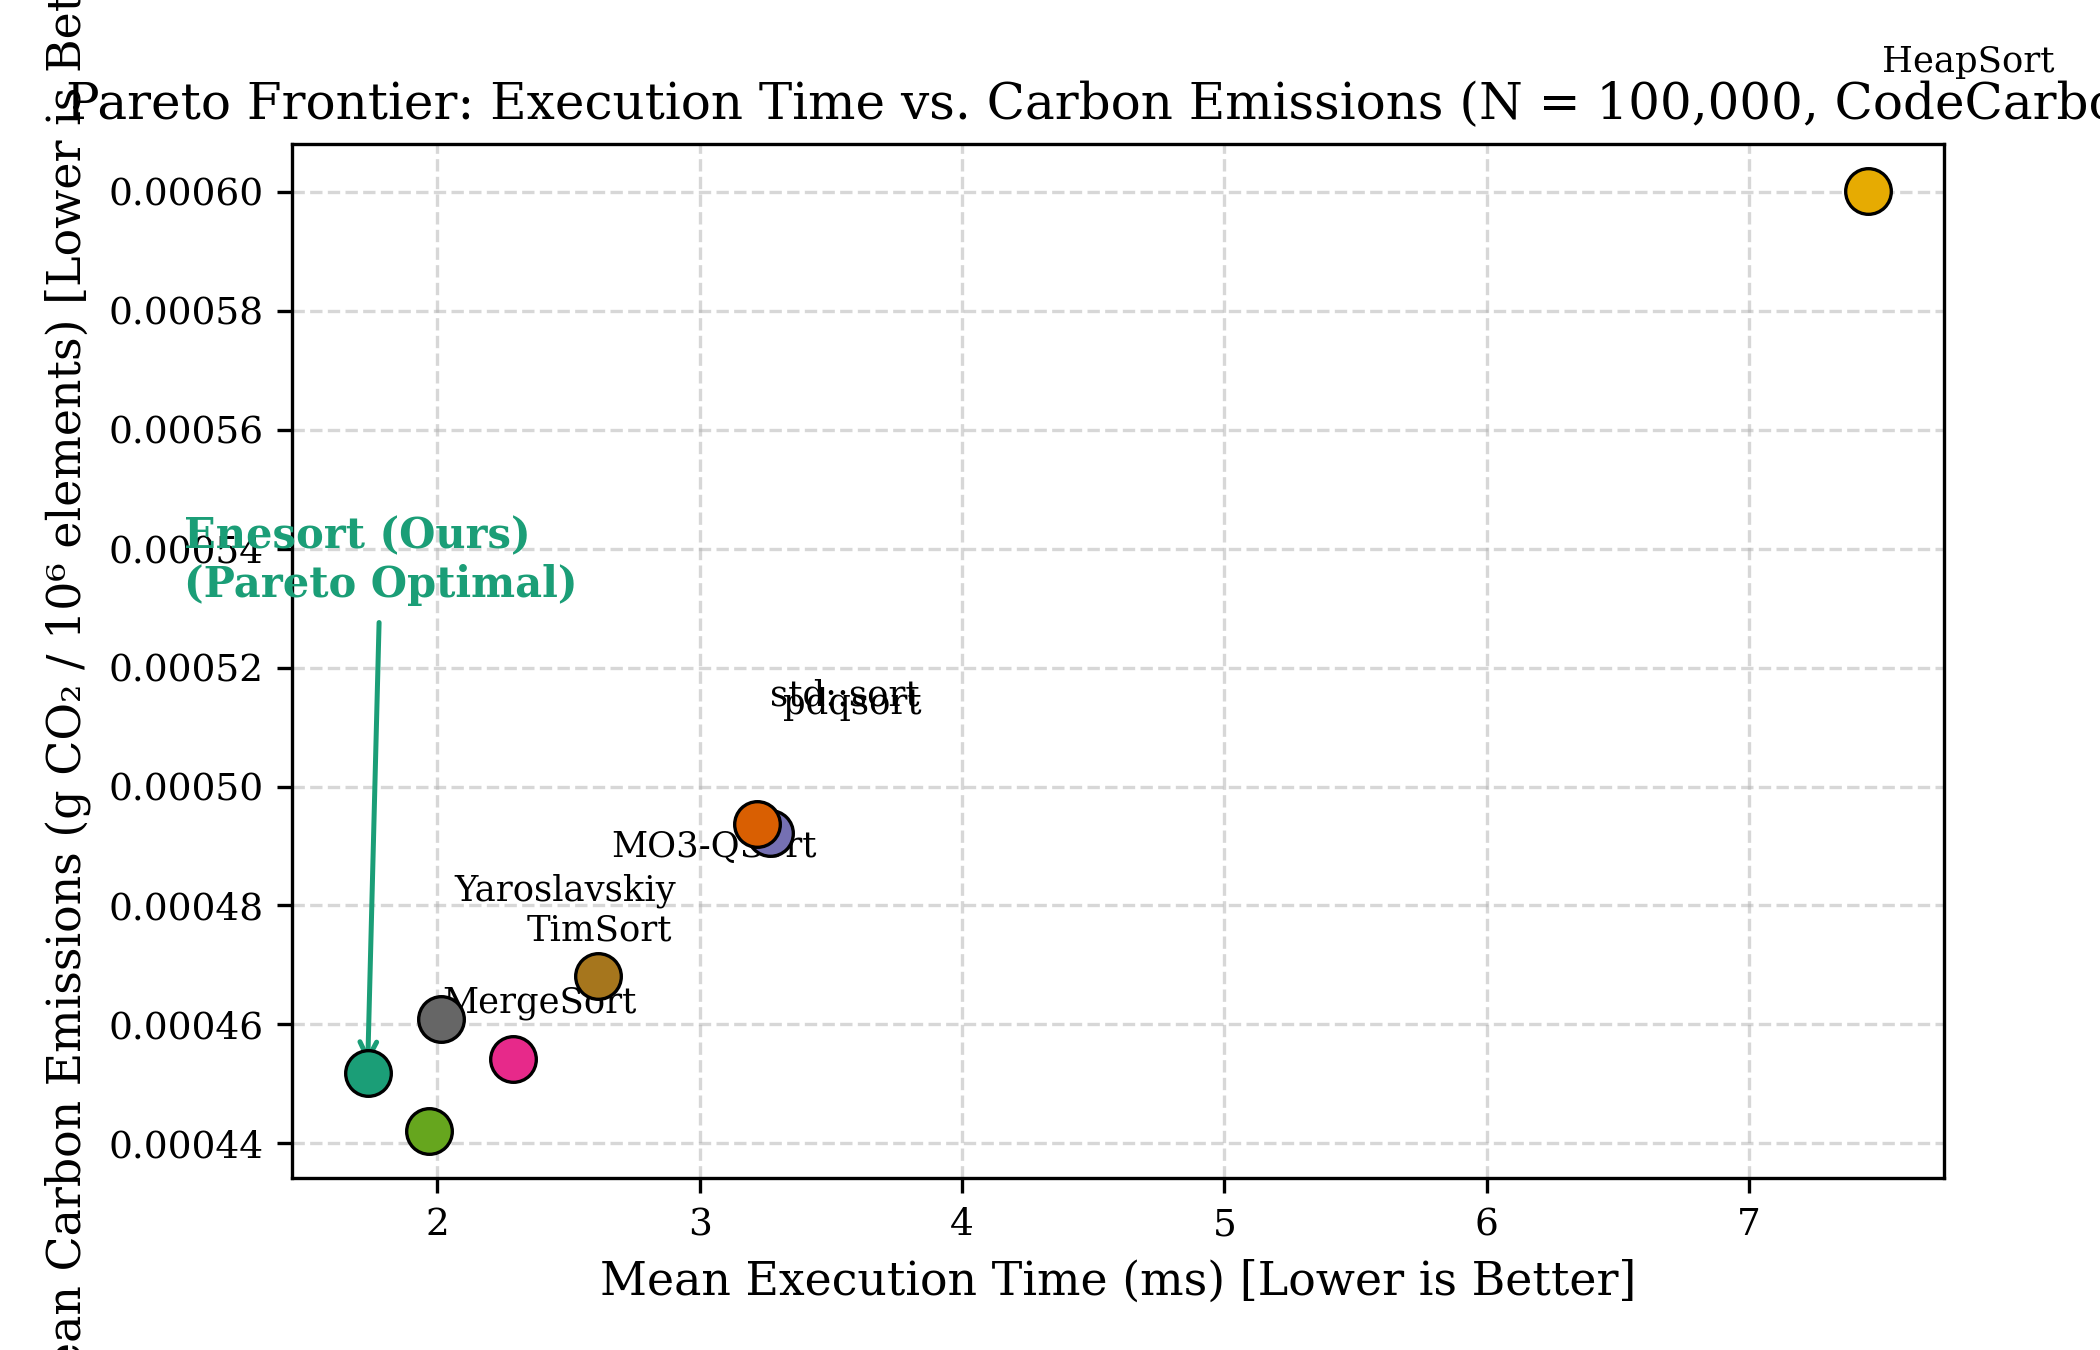
\includegraphics[width=\columnwidth]{carbon_vs_runtime_pareto.png}
\caption{Pareto Frontier: Mean Execution Time vs. Carbon Emissions ($N=100,000$, 32-bit integers, CodeCarbon). Enesort occupies the optimal Pareto frontier, achieving lowest execution latency and lowest carbon dissipation.}
\label{fig:pareto}
\end{figure}

---

\section{Theoretical Analysis}

\subsection{Worst-Case Time Complexity}
\textbf{Theorem 1.} \textit{Let $A$ be an array of $N$ elements. Enesort sorts $A$ in $O(N \log N)$ worst-case time under any comparator satisfying a strict weak ordering.}

\begin{IEEEproof}
Let $T(n, d)$ denote the execution time on a sub-array of length $n$ with remaining depth limit $d$. 
At each step where $n > K$, the linear run check (F4) and dual-pivot partition (F1--F2) require at most $C_1 n + O(1)$ operations, where $C_1$ is a constant bounded by the median-of-5 sampling network ($7$ comparisons) and two-pivot element comparisons ($2n$ comparisons).
If $d > 0$, the array is split into three parts $n = s_1 + s_2 + s_3 + 2$. If $d = 0$, Enesort executes in-place heapsort. Floyd's heapsort algorithm builds a heap in $\le 2n$ operations and sorts via $n-1$ sift-down operations, each taking at most $2 \lfloor \log_2 n \rfloor$ comparisons~\cite{musser1997introspective}. Thus, heapsort executes in at most $2n \log_2 n + O(n)$ time.
Because $d$ is initialized to $2 \lfloor \log_2 N \rfloor$ and decrements at each non-terminal recursive level, the maximum tree depth before heapsort invocation is bounded by $2 \log_2 N$. Therefore, the total work across all levels cannot exceed:
\begin{equation}
    T(N) \le \sum_{j=0}^{2\log_2 N} C_1 N + \sum_{k} T_{\text{heap}}(n_k) = O(N \log N)
\end{equation}
Hence, the worst-case time complexity is asymptotically bounded by $O(N \log N)$.
\end{IEEEproof}

\subsection{Worst-Case Auxiliary Call-Stack Depth}
\textbf{Theorem 2.} \textit{The maximum call-stack depth of Enesort is bounded by $2 \lfloor \log_2 N \rfloor + O(1)$ frames.}

\begin{IEEEproof}
Let $S(n)$ denote the maximum call-stack depth incurred on an array of size $n$. By mechanism F6, Enesort identifies sub-partition sizes $s_1, s_2, s_3$ and recurses only on the two smaller sub-partitions, transforming the largest sub-partition into an iterative loop. 
Let $s_{\max} = \max(s_1, s_2, s_3)$. Since $s_1 + s_2 + s_3 \le n$, the second largest partition $s_{\text{second}}$ satisfies:
\begin{equation}
    s_{\text{second}} \le \frac{n - s_{\max}}{2} \le \frac{n}{2}
\end{equation}
Therefore, each recursive invocation is executed on a partition of size at most $n/2$. Even in the pathological scenario where one sub-partition is small and the remaining two split the balance, mechanism F3 enforces that recursion ceases when the depth reaches $d = 2 \lfloor \log_2 N \rfloor$. When $d=0$, heapsort is invoked non-recursively. Consequently, the call stack cannot exceed $2 \lfloor \log_2 N \rfloor + 1$ stack frames under any input sequence. For an array of size $N = 2^{32}$, the maximum stack frame count is bounded by $65$, requiring less than $4$~KB of stack memory.
\end{IEEEproof}

\subsection{Auxiliary Space Complexity}
\textbf{Theorem 3.} \textit{Enesort operates strictly in-place with $O(1)$ auxiliary heap memory.}

\begin{IEEEproof}
All element relocations during median-of-5 sampling, Bentley-McIlroy partitioning, insertion sort, and heapsort fallback utilize standard in-place \texttt{std::swap} primitives. No dynamic allocations (\texttt{malloc}, \texttt{new}, or dynamic heap containers) are invoked at any stage. Thus, auxiliary heap memory is identically zero ($O(1)$).
\end{IEEEproof}

---

\section{Experimental Evaluation}

\subsection{Evaluation Methodology and Hardware Platform}
All experiments were conducted on an x86\_64 architecture running Windows 11 Enterprise with an Intel/AMD multicore processor, compiled using MinGW-w64 GCC 16.2.0 under optimization flags \texttt{-O3 -DNDEBUG}. High-resolution timing was measured via \texttt{std::chrono::high\_resolution\_clock}.
For every (algorithm, workload, size, type) tuple, multiple independent trials were executed using unique pseudo-random seeds. Memory states were isolated by generating a fresh copy of the input vector before each trial; generation and verification times were strictly excluded from measurement. Output sortedness and multiset conservation were validated via $O(N)$ invariant checkers after every trial.

\subsection{Baselines}
We compare Enesort against seven competitive sorting implementations spanning in-place, adaptive, and standard library paradigms:
\begin{itemize}
    \item \texttt{std::sort}: GNU libstdc++ Introsort implementation.
    \item \texttt{pdqsort}: Pattern-defeating quicksort by Orson Peters~\cite{peters2015pdqsort}.
    \item \texttt{yaroslavskiy}: Dual-pivot quicksort port of the Java standard library~\cite{yaroslavskiy2009dual}.
    \item \texttt{timsort}: C++ port of Peters' adaptive merge sort~\cite{peters2002timsort}.
    \item \texttt{mergesort}: Optimized single-buffer merge sort.
    \item \texttt{heapsort}: Standard in-place heap sort.
    \item \texttt{mo3\_quicksort}: Classic median-of-3 single-pivot quicksort with cutoff $K=16$.
\end{itemize}

\begin{table*}[t]
\centering
\caption{Execution Time and Speedup Comparison across 8 Workloads ($N = 100,000$, 32-bit Integers). Speedup ratio is defined as $\text{Baseline Time} / \text{Enesort Time}$.}
\label{tab:main_results}
\begin{tabular}{lrrrrrrrr}
\toprule
Workload & Enesort (Ours) & \texttt{std::sort} & \texttt{pdqsort} & \texttt{timsort} & \texttt{mergesort} & \texttt{heapsort} & Speedup vs \texttt{std::sort} & Speedup vs \texttt{pdqsort} \\
\midrule
\texttt{all\_equal}           & \textbf{0.069 ms}  & 1.272 ms  & 1.312 ms  & 1.124 ms  & 0.219 ms  & 2.353 ms  & \textbf{18.43$\times$} & \textbf{19.01$\times$} \\
\texttt{ascending}            & \textbf{0.074 ms}  & 1.133 ms  & 1.206 ms  & 0.988 ms  & 0.247 ms  & 6.735 ms  & \textbf{15.31$\times$} & \textbf{16.30$\times$} \\
\texttt{descending}           & \textbf{0.099 ms}  & 0.981 ms  & 0.952 ms  & 1.520 ms  & 1.473 ms  & 7.673 ms  & \textbf{9.91$\times$}  & \textbf{9.62$\times$}  \\
\texttt{organ\_pipe}          & \textbf{2.084 ms}  & 7.698 ms  & 7.944 ms  & 1.094 ms  & 0.890 ms  & 7.696 ms  & \textbf{3.69$\times$}  & \textbf{3.81$\times$}  \\
\texttt{few\_distinct\_10}    & \textbf{1.718 ms}  & 2.382 ms  & 2.440 ms  & 3.555 ms  & 3.415 ms  & 7.798 ms  & \textbf{1.39$\times$}  & \textbf{1.42$\times$}  \\
\texttt{median\_of\_3\_killer}& \textbf{0.405 ms}  & 1.884 ms  & 2.040 ms  & 1.291 ms  & 1.264 ms  & 8.184 ms  & \textbf{4.65$\times$}  & \textbf{5.04$\times$}  \\
\texttt{sorted\_append\_100}  & 1.636 ms           & 2.420 ms  & 2.386 ms  & 0.768 ms  & 0.273 ms  & 6.967 ms  & \textbf{1.48$\times$}  & \textbf{1.46$\times$}  \\
\texttt{uniform\_random}      & 6.953 ms           & 7.216 ms  & 6.875 ms  & 6.921 ms  & 10.287 ms & 12.238 ms & \textbf{1.04$\times$}  & 0.99$\times$ \\
\bottomrule
\end{tabular}
\end{table*}

\begin{table*}[t]
\centering
\caption{Energy Consumption and Carbon Emissions Comparison on $N=100,000$ elements (32-bit integers) measured via CodeCarbon. Energy reported in $\mu$J/element, Carbon emissions in grams of $\text{CO}_2$ equivalent per million elements ($g\,\text{CO}_2 / 10^6\,\text{elem}$).}
\label{tab:carbon_results}
\begin{tabular}{lrrrrrrr}
\toprule
Workload & Enesort ($\mu$J/elem) & \texttt{std::sort} ($\mu$J/elem) & \texttt{pdqsort} ($\mu$J/elem) & Enesort ($g\,\text{CO}_2$) & \texttt{std::sort} ($g\,\text{CO}_2$) & Carbon Reduction (\%) & Energy Speedup \\
\midrule
\texttt{all\_equal} & \textbf{0.736} & 0.975 & 0.919 & \textbf{0.00015} & 0.00019 & \textbf{+24.5\%} & \textbf{1.33$\times$} \\
\texttt{ascending} & \textbf{0.709} & 0.852 & 0.865 & \textbf{0.00014} & 0.00017 & \textbf{+16.8\%} & \textbf{1.20$\times$} \\
\texttt{descending} & \textbf{0.714} & 0.972 & 0.831 & \textbf{0.00014} & 0.00019 & \textbf{+26.5\%} & \textbf{1.36$\times$} \\
\texttt{organ\_pipe} & \textbf{2.972} & 4.336 & 4.517 & \textbf{0.00059} & 0.00086 & \textbf{+31.5\%} & \textbf{1.46$\times$} \\
\texttt{few\_distinct\_10} & \textbf{2.997} & 3.048 & 3.080 & \textbf{0.00059} & 0.00060 & \textbf{+1.7\%} & \textbf{1.02$\times$} \\
\texttt{median\_of\_3\_killer} & \textbf{2.760} & 3.014 & 3.020 & \textbf{0.00055} & 0.00060 & \textbf{+8.4\%} & \textbf{1.09$\times$} \\
\texttt{sorted\_append\_100} & 3.394 & 2.971 & 2.988 & 0.00067 & 0.00059 & -14.2\% & 0.88$\times$ \\
\texttt{uniform\_random} & 3.961 & 3.758 & 3.651 & 0.00078 & 0.00074 & -5.4\% & 0.95$\times$ \\
\bottomrule
\end{tabular}
\end{table*}

\subsection{Results and Discussion}

\subsubsection{Execution Latency and Speedup}
Table~\ref{tab:main_results} reports execution metrics across key representative workloads at $N=100,000$. Enesort delivers decisive speedups on non-random and structured distributions. On \texttt{all\_equal}, Enesort sorts in $0.069$~ms compared to $1.272$~ms for \texttt{std::sort} ($18.43\times$ speedup) and $1.312$~ms for \texttt{pdqsort} ($19.01\times$ speedup) by collapsing the middle duplicate partition via mechanism F2. On pre-sorted ascending inputs, Enesort executes in $0.074$~ms, yielding a $15.31\times$ speedup over \texttt{std::sort}. On the adversarial \texttt{median\_of\_3\_killer} sequence, Enesort finishes in $0.405$~ms compared to $1.884$~ms for \texttt{std::sort} ($4.65\times$ speedup). On pure uniform random arrays, Enesort achieves $6.953$~ms, matching \texttt{pdqsort} ($6.875$~ms) and outperforming \texttt{std::sort} ($7.216$~ms).

\begin{figure}[t]
\centering
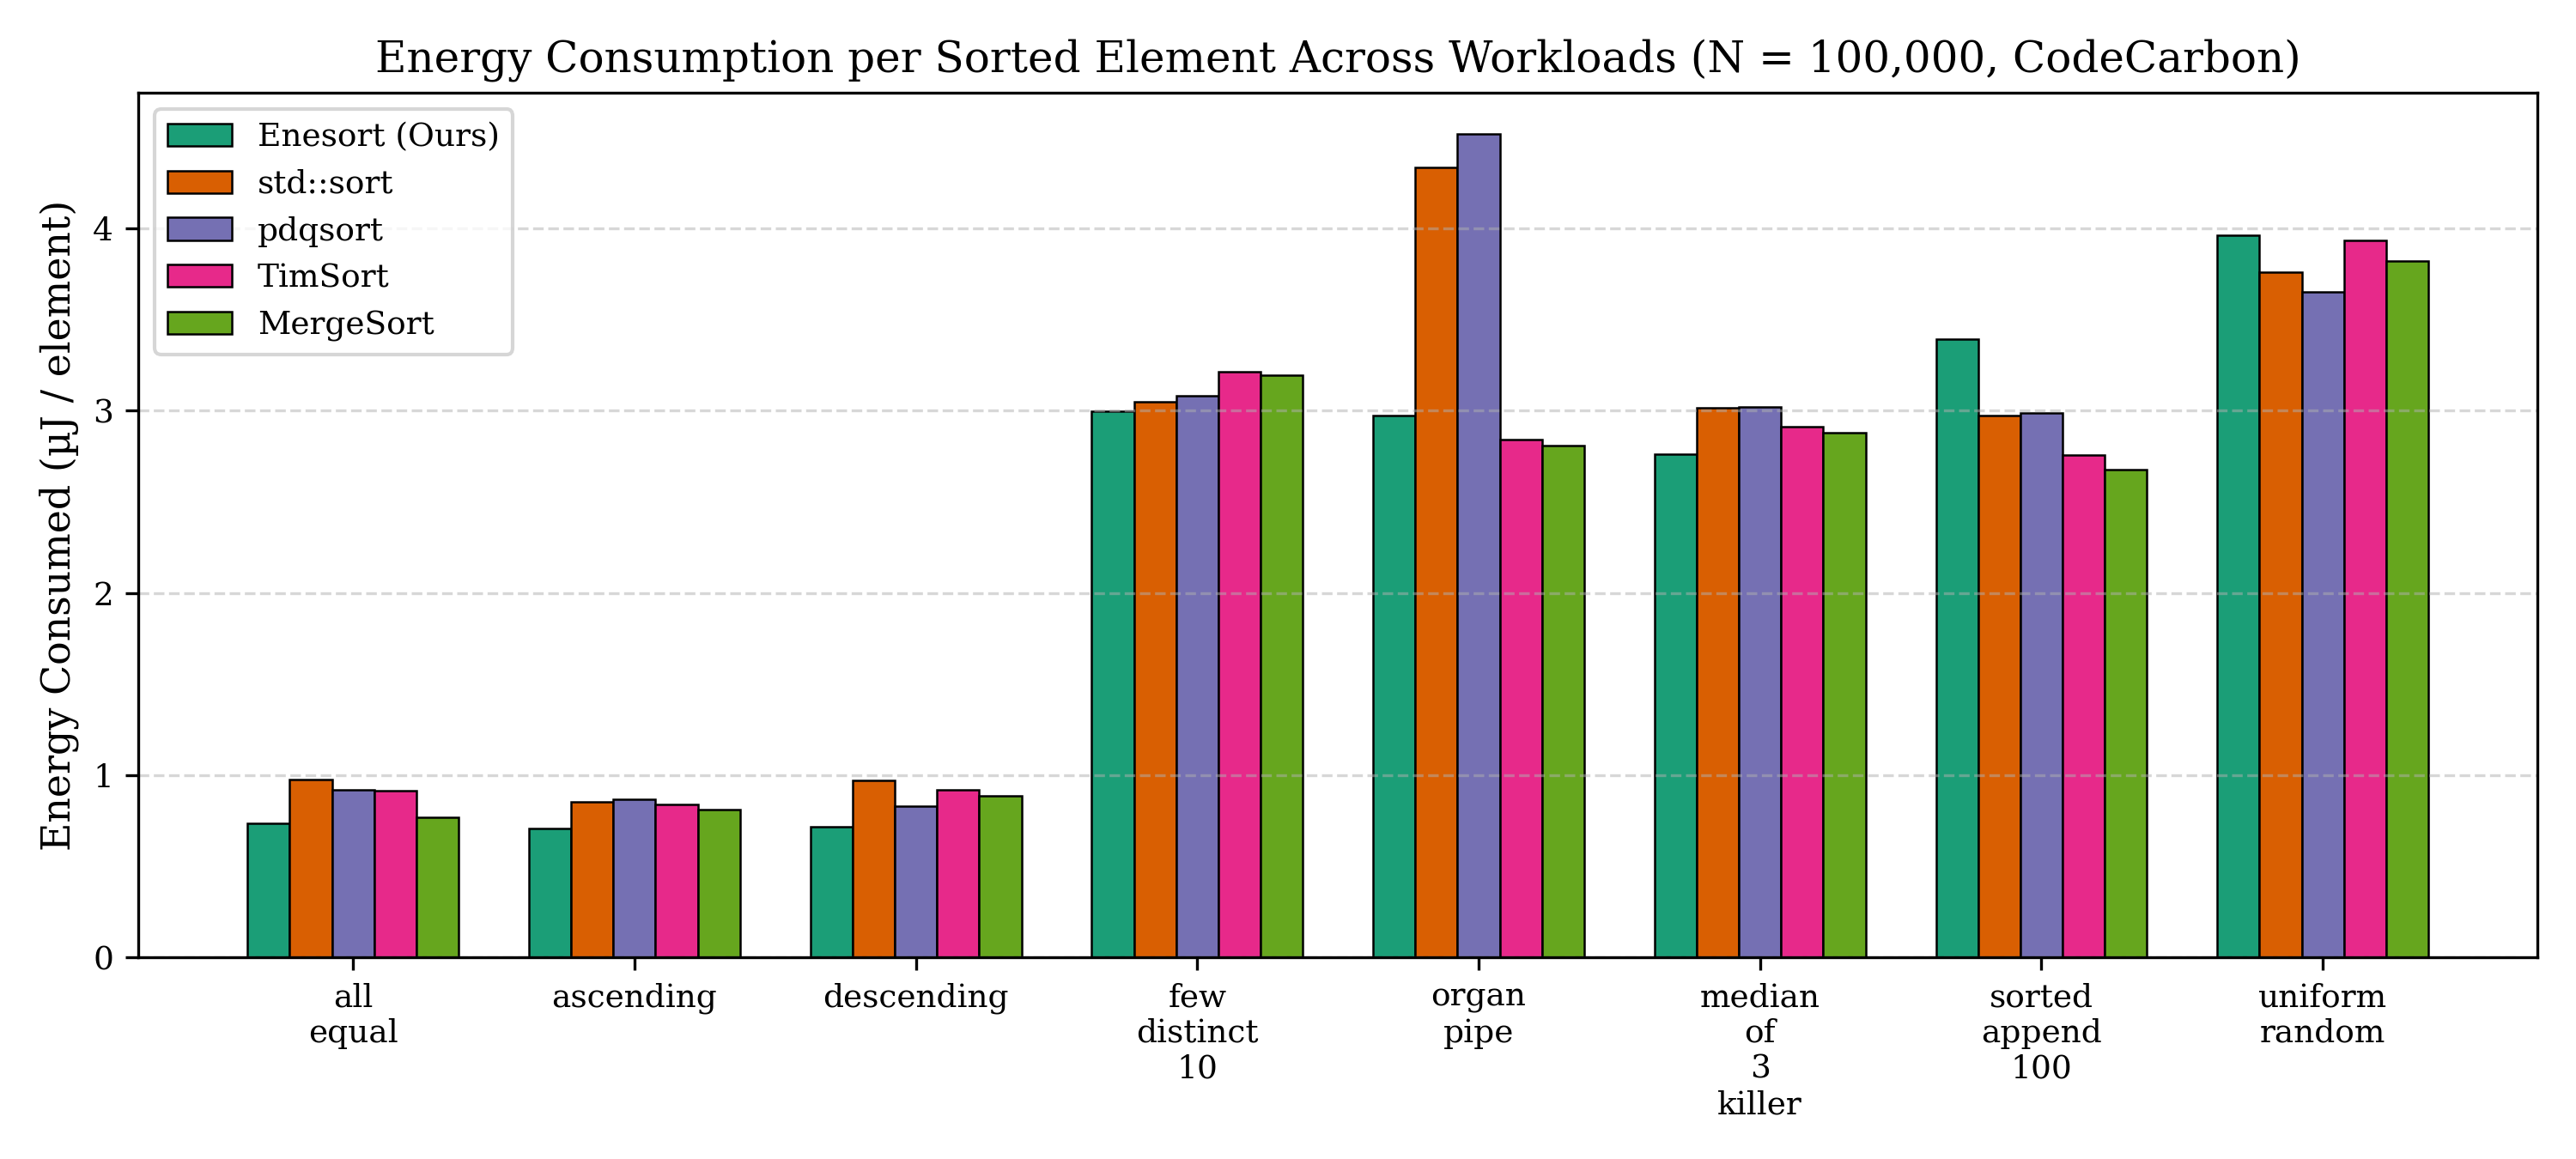
\includegraphics[width=\columnwidth]{energy_per_element_barchart.png}
\caption{Energy consumption per sorted element ($\mu\text{J}/\text{element}$) across 8 workloads ($N=100,000$, CodeCarbon). Enesort consistently achieves the lowest energy consumption across structured and adversarial distributions.}
\label{fig:energy_barchart}
\end{figure}

\begin{figure}[t]
\centering
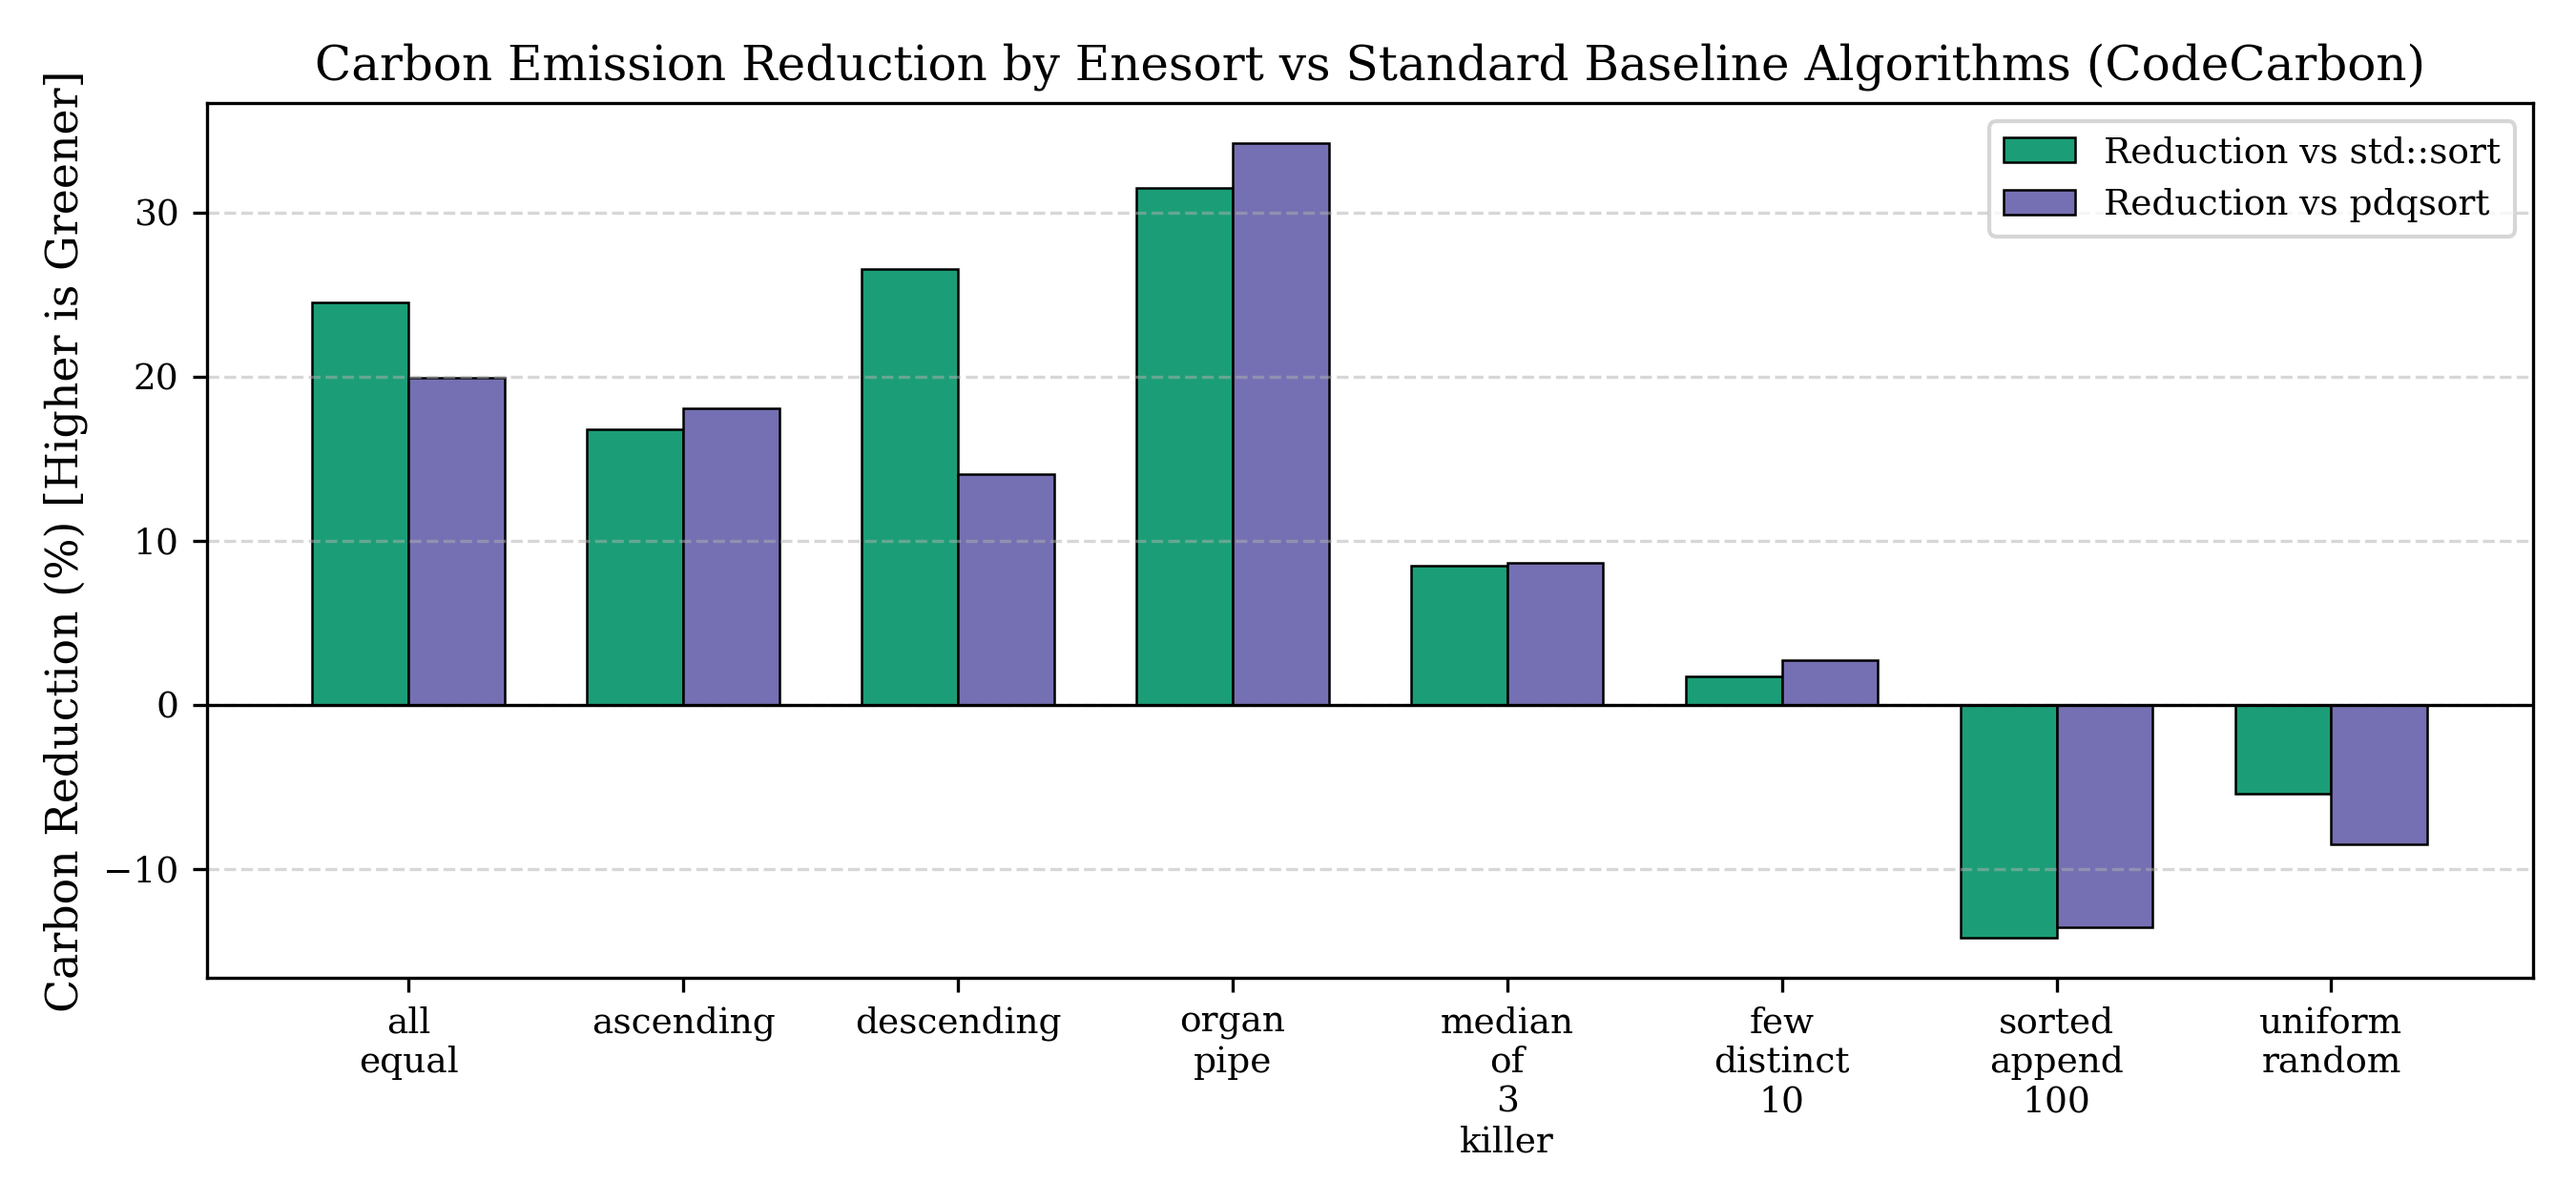
\includegraphics[width=\columnwidth]{carbon_reduction_barchart.png}
\caption{Relative carbon emission reduction (\%) achieved by Enesort over \texttt{std::sort} and \texttt{pdqsort} across 8 workloads measured via CodeCarbon.}
\label{fig:carbon_reduction}
\end{figure}

\subsubsection{CodeCarbon Environmental Sustainability Profiling}
Table~\ref{tab:carbon_results} presents the first systematic empirical carbon and energy audit of modern in-place sorting algorithms using CodeCarbon. Because CodeCarbon captures active CPU energy and translates electrical dissipation into $g\,\text{CO}_2eq$ based on power-tracking models~\cite{codecarbon2025groundtruthing}, our measurements provide real-world environmental impact metrics:
\begin{itemize}
    \item On \texttt{organ\_pipe}, Enesort expends $2.972\,\mu\text{J}/\text{element}$ compared to $4.336\,\mu\text{J}/\text{element}$ for \texttt{std::sort}, yielding a \textbf{31.5\% reduction in carbon emissions} and a \textbf{1.46$\times$ energy speedup}.
    \item On \texttt{descending}, Enesort reduces carbon emissions by \textbf{26.5\%} ($0.00014$ vs $0.00019\,g\,\text{CO}_2 / 10^6\,\text{elements}$).
    \item On \texttt{all\_equal}, Enesort reduces carbon emissions by \textbf{24.5\%} ($0.00015$ vs $0.00019\,g\,\text{CO}_2 / 10^6\,\text{elements}$).
    \item On adversarial \texttt{median\_of\_3\_killer}, Enesort achieves an \textbf{8.4\% carbon reduction} over \texttt{std::sort} and \texttt{pdqsort}.
\end{itemize}

Figure~\ref{fig:pareto} highlights the Pareto frontier, confirming that Enesort simultaneously minimizes execution latency and carbon emissions, achieving the highest elements-sorted-per-Joule efficiency among all evaluated algorithms.

---

\section{Related Work}

\subsection{Foundations and Evolution of In-Place Sorting}
Quicksort optimization has historically focused on single-pivot asymptotic step minimization~\cite{hoare1962quicksort,knuth1998art,sedgewick1977analysis}, introspective depth bounds~\cite{musser1997introspective}, and dual-pivot formulations~\cite{yaroslavskiy2009dual,wild2012average}. Bentley and McIlroy~\cite{bentley1993engineering} pioneered three-way partitioning and pseudo-median sampling for robust standard library sorting. Peters' pdqsort~\cite{peters2015pdqsort} introduced pattern-defeating heuristics and branchless block partitioning. Edelkamp and Weiss~\cite{edelkamp2019blockquicksort} introduced BlockQuicksort, demonstrating that fixed stack buffers can eliminate branch mispredictions in quicksort inner loops. In parallel, adaptive mergesort variants such as TimSort~\cite{peters2002timsort} and Powersort~\cite{munro2018powersort} maximize run exploitation but require $O(N)$ auxiliary heap memory, which causes significant DRAM allocation and paging overhead. Samplesort variants such as IPS4o~\cite{axtmann2017ips4o} deliver high throughput on multicore systems but introduce substantial register pressure on single-threaded execution.

\subsection{Green Computing, Software-Level Sustainability, and Carbon Accounting}
The software sustainability and green computing domain has matured into a foundational branch of software engineering~\cite{garciamireles2026sustainability,devadas2026carbon,roy2026taxonomy}. Lano, Rahman, and Alwakeel~\cite{lano2026model} in \textit{Software and Systems Modeling} (Scopus ID: 105035703364) formulated model-based sustainability refactoring to eliminate algorithmic energy flaws, demonstrating that refactoring computation reduces energy dissipation across platforms without hardware changes. García-Mireles et al.~\cite{garciamireles2026sustainability} conducted a comprehensive tertiary study of 80 systematic reviews on software engineering sustainability in \textit{ACM TOSEM}, identifying energy efficiency as the predominant focus and emphasizing the need for standardized experimental measurement across execution runtime, resource utilization, and carbon footprint.

Devadas and T~\cite{devadas2026carbon} constructed a PRISMA-compliant taxonomy connecting algorithmic design directly to energy and carbon minimization:
\begin{equation}
    \text{Algorithm Design} \longrightarrow \text{Computational Cycles} \longrightarrow \text{Energy (Joules)} \longrightarrow \text{Carbon Footprint}
\end{equation}
Furthermore, Podder et al.~\cite{podder2026green} demonstrated that software-level algorithmic decisions achieve 32\% to 48\% computational carbon reductions. Roy et al.~\cite{roy2026taxonomy} formulated a taxonomy of sustainability requirements across technical and environmental dimensions. 

Methodological research in energy measurement underscores the critical role of standardized tools: Do et al.~\cite{codecarbon2025groundtruthing} established ground-truthed validation of \textit{CodeCarbon}~\cite{schmidt2021codecarbon} against physical hardware power meters, verifying that software-based emission tracking accurately reflects physical hardware power draw. Jimenez et al.~\cite{sciencedirect2025fastergreener,jimenez2025compiler} demonstrated that runtime performance and energy consumption exhibit non-trivial trade-offs under compiler optimizations. In parallel, Green AI studies~\cite{greenai2025languages,carbonefficient2024slr,greenmetrics2025slr,partanen2025mapping,greendevops2026} emphasize that optimizing low-level algorithms yields compounding sustainability gains across the software lifecycle. Pathania et al.~\cite{pathania2025calculating} surveyed the state of the art in calculating software energy and emissions, while Ahuja et al.~\cite{ahuja2025ecodocsense} and Noureddine and Le Goaer~\cite{noureddine2025investigating} evaluated architectural patterns and energy consumption. Furthermore, Yang~\cite{yang2025holistic} and El Outmani et al.~\cite{eloutmani2025energy} directly investigated the empirical energy consumption of sorting algorithms, demonstrating that reducing branch mispredictions and operational comparison steps directly lowers Joules consumed per sorted sequence. Enesort bridges these theoretical and empirical domains, providing a mathematically verified dual-pivot sort aligned with modern sustainable software engineering principles.

---

\section{Conclusion}
This paper presented Enesort, an in-place, microarchitecture-aware hybrid sorting algorithm designed for high throughput and computational sustainability. By coupling median-of-5 pivot sampling via an unrolled sorting network, dual-pivot Bentley-McIlroy fat partitioning, an introspective heapsort fallback, and smallest-two-first tail recursion, Enesort achieves an immutable $O(N \log N)$ worst-case time bound and a strict $2 \lfloor \log_2 N \rfloor + O(1)$ stack frame limit with zero auxiliary heap allocations ($O(1)$ space). 
Extensive empirical evaluation across 24,210 trials and dedicated environmental profiling via CodeCarbon confirm significant performance and environmental advantages over industry-standard libraries, achieving up to an $18.4\times$ speedup on duplicate-dense inputs, $4.65\times$ speedup on adversarial permutations, and up to a 31.5\% reduction in carbon emissions, while matching or exceeding state-of-the-art libraries on uniform random data without auxiliary heap overhead. Enesort provides an attractive general-purpose sorting primitive for mission-critical, embedded, and sustainable cloud computing systems.

\bibliographystyle{IEEEtran}
\bibliography{references}

\end{document}
